%!TEX root = ../thesis.tex
\chapter{Methods}
\label{ch:methods}

\todo{approach section, use model project overview graphic (?)}
The key idea of our approach is to use the versatile MATLAB platform to create an easily expandable model of a hexapod robot, aiming to accelerate future research.
By basing our work on this platform we will in the future be able to incorporate concepts from different domains with a more streamlined development process and less development time, given the provided toolboxes.
In this chapter we detail the approach and methodology used to address the objectives we defined in the introduction.
As the controller and RL setup both depend on a solid, well-working model, we will first describe the representation of the hexapod we created in Simulink.
We will then continue with a description of the static gait motion controller, including trajectory generation and inverse kinematics solver.
The chapter concludes with the explanation of our reinforcement learning setup used to train an agent on leg coordination/ gait generation.


\section{Simulink Model}

\begin{figure}[h]
	\centerline{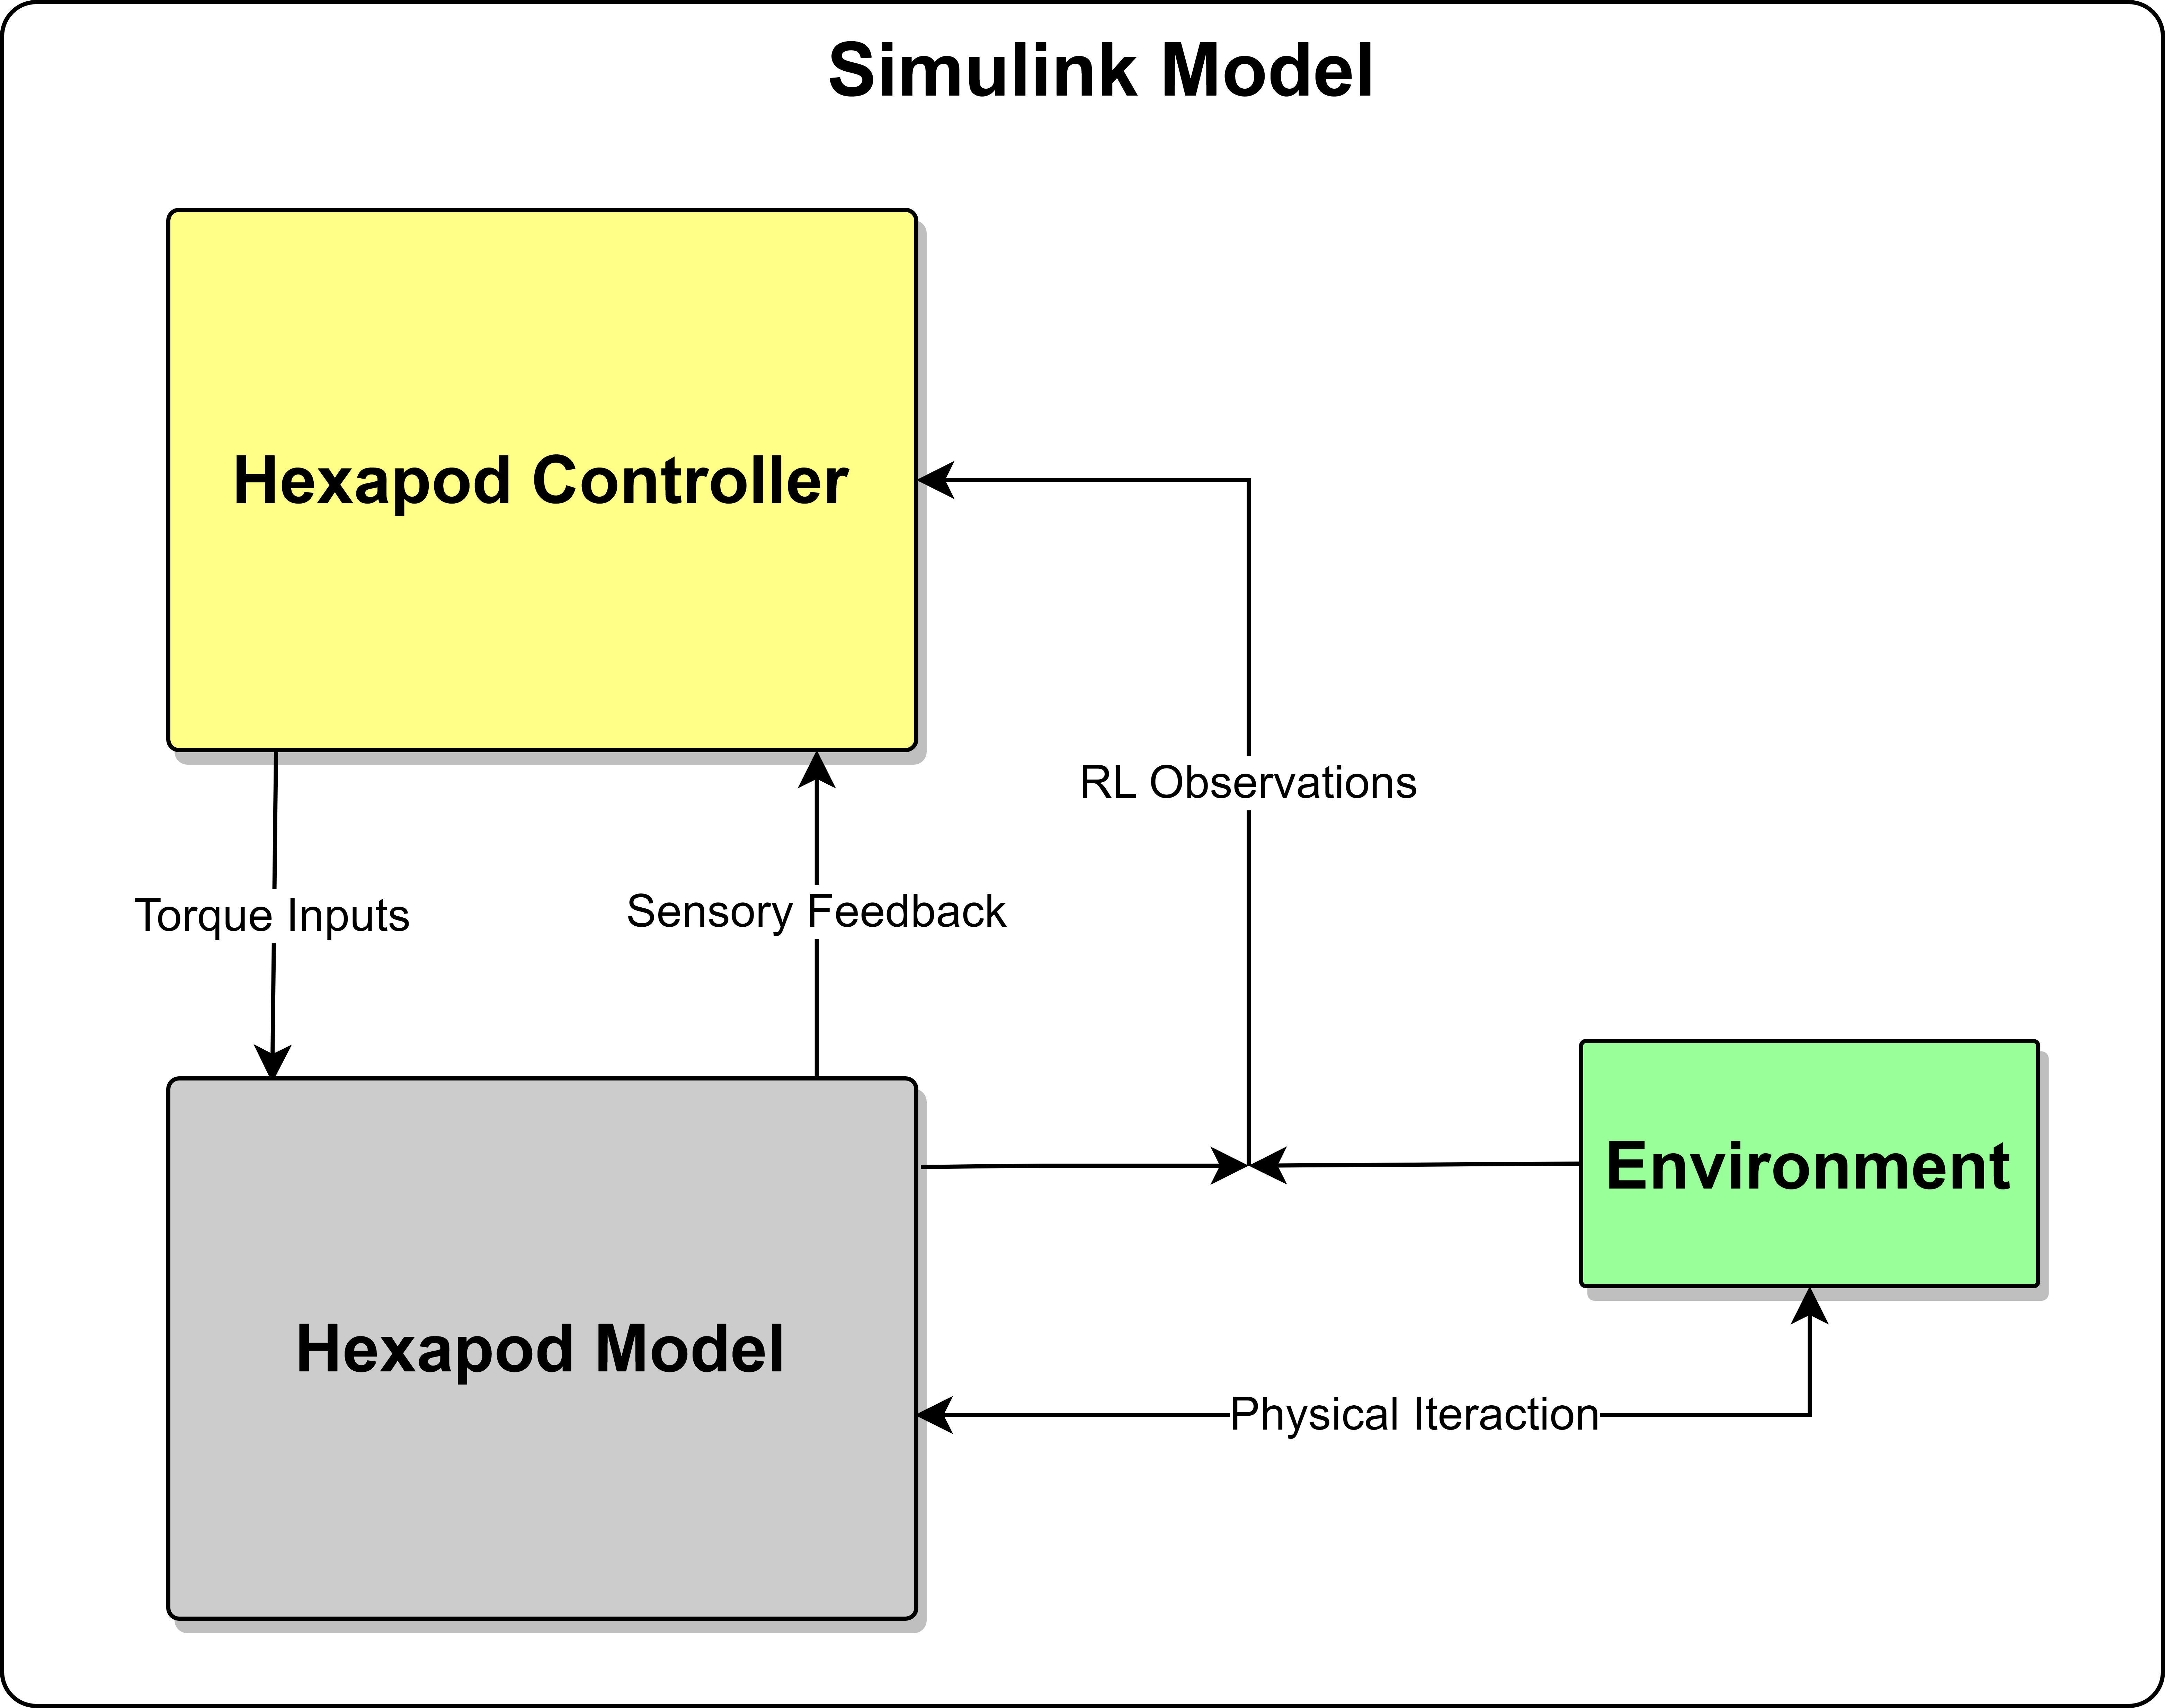
\includegraphics[scale=0.035]{HexapodModel_Overview}}
	\caption{Simulink Model Overview}
	\label{figure: Simulink Model Overview}
\end{figure}
\todo{MALTE: Change name of "Physical Hexapod Model in graphic and everywhere else"}

Taking a top-down perspective on the Simulink model as depicted in \ref{figure: Simulink Model Overview}, it is distinctly divided into 3 separate components, the hexapod, the controller and the environment.
Being responsible for conducting the hexapods movement, the controller is, on a abstract level, responsible for deciding on the the speed, gait and direction of the robots movements.
On the lowest level this is accomplished by instructing the hexapod which torque has to be applied to each of its joints. 
The hexapod and the environment represent the components which physically interact with each other during the simulation.
Responding upon the commands received by the controller, the hexapod applies the torque values at each simulation step and returns sensory feedback to the controller.
This feedback is then used to adjust the commands which the controller will send during the next time step.
The hexapod takes all of these actions inside of the environment, all while interacting with it.
Additionally, if a RL agent is supposed to be trained, both the hexapod and the environment provide specific observations to the controller, which are used as inputs to the agent or to compute the reward function. 


\subsection{Model of the Hexapod}
The hexapod model we develop in this thesis is based on the \textit{PhantomX MK4} hexapod distributed by \textit{Trossen Robotics}.
The company provides a digital model of this robot in the form of an .urdf file which can be obtained from their Github page \parencite{interboticsGithub}.
URDF (\textbf{U}nified \textbf{R}obotics \textbf{D}escription \textbf{F}ormat) is a common file format for describing the physical and kinematic properties of a robot or robotic component.
It provides a standardized and structured way to define the connections between joints and links, the visual properties and collision geometry of each link as well as parameters such as mass and inertia \parencite{matlabURDFDocumentation}.
The geometry is provided in a separate folder in the form of CAD-files which are then referenced by the urdf.

The \textit{PhantomX MK4} follows the common architecture mentioned in \ref{sec: Hexapods}, meaning each leg has 3 joints and segments, totalling 18 DoFs.
Concerning the joint orientations, the \textalpha-joints movement plane lies is parallel to the ground while the \textbeta- and \textgamma-joint are restricted to a plane perpendicular to the ground, also in accordance to mentioned architecture.
The robot is axisymmetric towards its central axis(pointing in the movement direction) and the front and hind leg pairs are equally spaced from the middle leg pair.
The middle legs are attached to the thorax slightly further away from the central axis than the front and back legs.
A 3D model of the hexapod can be seen in Fig. \ref{figure: PhantomX 3D model}.

To import the model into the Simulink environment, we us a MATLAB-provided function to convert it from a urdf-file into a Simulink block diagram.
This process works automatically and results in a physically accurate Simulink representation without having to manually re-model the robot.
The representation consists of blocks from the Simscape library, more specifically joints, rigid transforms and coordinate frames to describe the robots kinematic chains, and rigid bodies to represent the individual links geometry and physical parameters.

\begin{figure}[h]
	\begin{subfigure}{.5\textwidth} % this sets the figure to be max half the width of the page
		\centering
		% include first image
		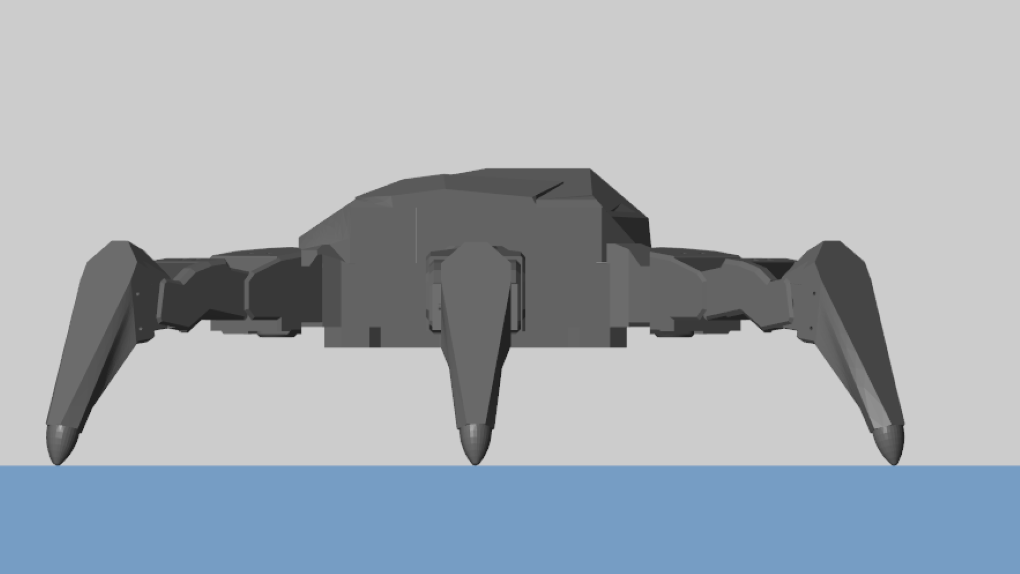
\includegraphics[width=.9\linewidth]{PhantomX_MK4_SideView}  % this sets the image to fill 90% of the available space -> 45% of the line width in total. 
		\caption{}
		\label{figure: PhantomX Side View}
	\end{subfigure}
	\begin{subfigure}{.5\textwidth}
		\centering
		% include second image
		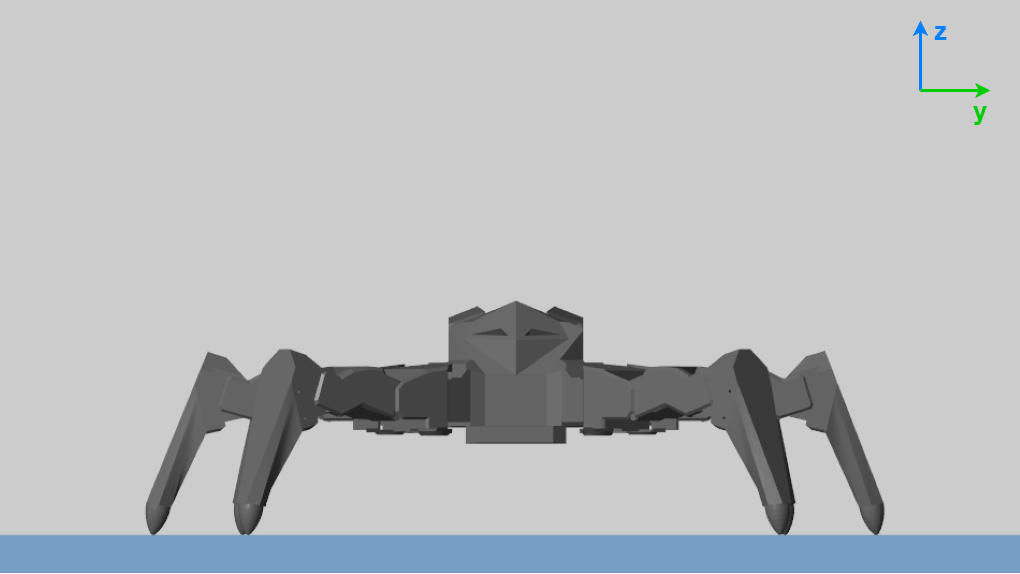
\includegraphics[width=.9\linewidth]{PhantomX_MK4_FrontView}  
		\caption{}
		\label{figure: PhantomX Front View}
	\end{subfigure}
	
	\label{fig:fig}
	\begin{subfigure}{\textwidth}
		\centering
		% include third image
		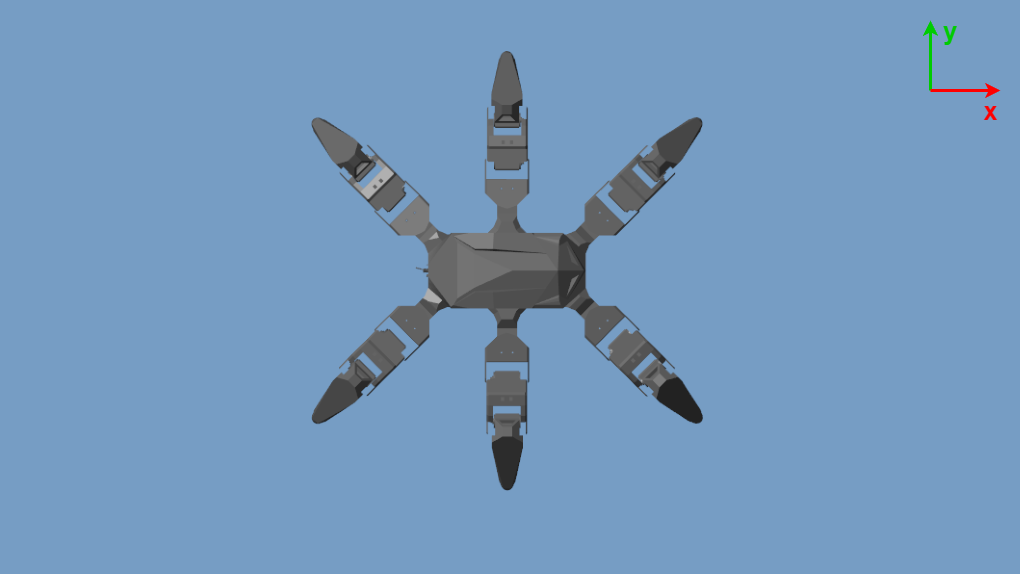
\includegraphics[width=.45\linewidth]{PhantomX_MK4_TopView}   % this width should be half of the width of the other two images
		\caption{}
		\label{figure: PhantomX Top View}
	\end{subfigure}
	\caption[]{3D model of Trossen Robotics PhantomX MK4}
	\label{figure: PhantomX 3D model}
\end{figure}
\todo{get each image into list of figures, but exclude complete figure}

To be able to use the imported hexapod as a development platform we have to modify and expand the raw Simulink model as it does not provide any means to control it or receive feedback.
We reorganise and encapsulate logical groups, specifically the thorax and the individual legs, into library subsystems.
This enables us to propagate changes faster, as we only have to edit the library component instead of each existing instance.
As a side effect, this given the Simulink model a much more cleaned up and easier to understand appearance.
To be able to control each joint and receive sensory feedback from it, we enable the so called \textit{direct torque input} as well as the \textit{position} and \textit{acceleration} sensor readings on each joint block.
Trying to prevent increasing the models complexity to quickly, we do not model the physical servo motor attached to each joint and instead use the instantaneous torque application.
the joint block also allows for physical parameters to be modified, such as internal friction, dampening or spring stiffness.
We combine the 3 torque values and position/ acceleration readings of each leg into an input and output bus signal.
A view inside of the leg subsystem is given in \ref{figure: Hexapod Leg}, the subsystem block itself with its torque input and sensory feedback output buses can be seen in \ref{figure: Hexapod Model Overview} as part of the complete hexapod model.

\begin{figure}[h]
	\centerline{\includesvg[scale=0.55]{Simulink/Simulink_PhysicalHexapodOverview}}
	\caption{Overview of the Simulink Hexapod Model}
	\label{figure: Hexapod Model Overview}
\end{figure}

\begin{figure}
	\centerline{\includesvg[scale=0.5]{Simulink/Simulink_HexapodLegOverview}}
	\caption{Simulink model of the Hexapod Leg subsystem}
	\label{figure: Hexapod Leg}
\end{figure}

To enable the robot to physically interact with its surroundings, we enable the collision geometry on each of the models rigid bodies.
In Simscape, collision modelling involves establishing connections between a rigid body, and any other rigid body it should be able to interact with in a collision scenario, via Simscapes's \textit{Spatial friction force} block.
The block allows to modify the coefficients of static and dynamic friction, elasticity and dampening.\todo{does dampening exist in block ?}
An example of how this block can be utilized is shown in \ref{figure: Simscape Bouncing Ball Example}.
As collision detection is computationally relative expensive, we refrain from modelling robot self collisions and focus only on the interaction between robot and environment.
This means that the hexapods links can only collide with the ground plane but not with each other.
We realise this can potentially create discrepancies between simulation and real world, but as we initially only model predefined leg trajectories, which can be proven to not intersect, we are willing to give up a bit of realism in favour of faster simulations.

From a top level perspective, the modified robot model is represented by a single \textit{Hexapod} subsystem block, which receives the torques to be applied as input and outputs sensory information about each joint.
All of the internal joint parameters and friction coefficients used to model collisions are given in the tables \ref{table: Joint parameters} and \ref{X}.
The joint parameters were already mostly given by the urdf specification, while we adapted other parameters from \parencite{trotta2022walking} and \parencite{AUTHOR2}.
\todo{Find source again}
To summarize, we converted the provided hexapod model into a Simulink model, compartmentalized it and added sensing and actuation capabilities to the robots legs.
In addition we made most of the models internal parameters accessible and modifiable within the MATLAB-script \textit{simulation\_setup.m}.



\begin{comment}
The  thorax is represented by a rigid body and a main coordinate frame.
Each of the robots legs consists of 3 rigid bodies(coxa, femur and tibia) which are connected to each other by 2 joints.
A third joint then attaches the coxa and the leg as a whole to the main body.
Like the leg of an insect, the movement plane of the joint connecting coxa and thorax is parallel to the ground and orthogonal towards the other two joints.
Each of the joints used has 1 (rotational) DoF.
To position each rigid body and joint correctly, rigid transformations are used to translate and rotate each component.

As mentioned above, joints can receive as input a torque to be applied and can output sensory data, such as the joints position, velocity and acceleration. 
\end{comment}


\begin{table}
	\centering
	\begin{tabular}{| l | c | c |}
		\hline
		\textbf{Parameter} & \textbf{Value} & \textbf{Unit}\\
		\hline
		\hline
		Spring stiffness & 0 & $\frac{N}{m}$\\
		
		Damping & 0 &  $\frac{N \cdot s}{m}$\\
		
		Spring stiffness (joint boundary) & 0 & $\frac{Nm}{\text{deg}}$ \\
		
		Damping coefficient (joint boundary) &  0 & $\frac{Nm \cdot s}{\text{deg}}$\\
		
		Transit region width (joint boundary) & 0 &  deg\\
		\hline
	\end{tabular}
	\caption{Internal joint parameters}
	\label{table: Joint parameters}
\end{table}

\todo{"Gait Self-learning for Damaged Robots Combining Bionic Inspiration and Deep Reinforcement Learning" for parameters of hexapod}

\begin{table}
	\centering
	\begin{tabular}{| l | c | c |}
		\hline
		\textbf{Parameter} & \textbf{Value} & \textbf{Unit} \\ 
		\hline
		\hline
		Stiffness & $1 \times 10^6$ & $\frac{N}{m}$ \\
		
		Damping & $1 \times 10^6$ & $\frac{N\cdot s}{m}$ \\
		
		Transition region width & $1 \times 10^{-3}$ & $m$ \\
		
		Static friction coefficient &  0.9 & $-$ \\
		
		Dynamic friction coefficient &  0.8 & $-$ \\
		
		Critical velocity & $1 \times 10^{-3}$ & $\frac{m}{s}$ \\
		\hline
	\end{tabular}
	\caption{\textit{Spacial contact force} parameters similar to  \cite{trotta2022walking}}
	\label{table: Spatial contact force}
\end{table}

%In this thesis we only utilize the sensor information about the current joint positions, but to allow for further expansions on the model, such as optimizing for minimal energy consumption, joint velocity and acceleration are provided as well.
%It should be noted, that integrating the joint position over time would implicitly yield the same result, but we decided for ease of use to include this data explicitly.


\subsection{Environment}
To validate the hexapod model and to provide a place for the robot to learn coordination strategies for its legs, we construct a simple test environment.
The environment at this point only consists of a horizontal plane, but can expanded to include more complex terrain with little effort.
Some examples which we experimented with, but did not utilise for testing or training so far, include inclined planes and also small obstacles on the ground.
As Simscape itself only provides basic geometric objects but allows for the use of .stl files to define the shape of objects, complex terrain such as irregular, uneven surfaces can be imported with relative ease.

In addition to being the testing ground of the hexapod model, the environment also acts as part of the reinforcement learning process.
Similar to \ref{figure: RL Illustration}, the environment provides observations to the RL agent and calculates a reward signal, based on the agents performance \todo{As of now not represented in the model, reward is part of controller}.
It does not however directly receive actions from the agent, as the hexapod, to which the actions are applied to by the RL agent, is its own subsystem.
If we would define the environment in a manner analogous to \ref{figure: RL Illustration}, we would have to include both the environment subsystem and the hexapod subsystem as part of the "RL" environment.
For obvious reasons such as modularity and clarity of model we choose not to adapt this.

\subsection{Locomotion Controller} \label{subsec: Locomotion controller}
The controller is responsible for the hexapods locomotion.
It controls the movement of the robots legs according to an internally defined gait pattern.
As inputs, the controller receives the sensor data from the hexapod model.
According to the internally defined gait pattern and the received data input, the controller computes the torques to be applied to each joint of the hexapod.
The controller subsystem can be described as a feedback control system, as it receives information about the process it controls and takes this feedback into account when generating new commands to steer the process.

\begin{figure}
	\centerline{\includegraphics[scale=0.03]{HexapodController}}
	\caption{Controller Overview}
	\label{figure: Controller Overview}
\end{figure}

A abstract diagram of the controller subsystem can be seen in Fig. \ref{figure: Controller Overview}.
As the legs move independently from one another, the controller consists of 6 separate control units, each responsible for controlling one of the six legs.
These units receive sensory information from the leg joints as input and compute the torques to be applied to the joints as output.
A legs control unit receives the desired frequency of the swing-stance cycle ($f_{c}$), the duty-cycle percentage ($P_{swing}$) and the swing-initiation signal of the respective leg ($s_i,\ i \in \{1,...,6\}$) as coordination inputs.
The frequency $f_{c}$ defines how often the swing-stance cycle should be repeated per second, $f_{c} = 0.5 \text{ Hz}$ for example corresponding to one cycle every 2 seconds.
$P_{swing}$ describes the proportion of the swing (duty) phase in relation to a whole cycle \parencite{qiu2023adaptive} and can be expressed by: 

\begin{equation}
P_{swing} = \frac{T_\text{sw}} {T_\text{st} + T_\text{sw}}
\end{equation}
where $T_\text{sw}$ and $T_\text{st}$ are the durations of the swing and stance phase respectively given as:
\begin{equation}
T_\text{sw} = \frac{P_\text{swing}}{f_c}, \quad T_\text{st} = \frac{1-P_\text{swing}}{f_c}
\end{equation}

A 50\% duty cycle corresponds to swing and stance being of equal length, both taking up exactly half a cycle time.
The swing initiation signal $s_i \in \{0,1\}$ for each of the six legs ($i \in \{1,...,6\}$) indicates to the control unit whether to initiate the swing phase ($s_i = 1$), independent of the legs position in its cycle.
$s_i = 0$ simply tells the control unit to continue on with the current cycle execution.
The control units also receive a movement direction vector as an additional input.
This vector points in the direction in which the robot is supposed to move.
All these inputs can either be received from a static gait definition, in which the parameters for each leg are statically configured, or can be provided by a reinforcement learning agent.

The Simulink RL Agent, a standard library block and separate component of the controller subsystem, receives the current time steps observations $o_t$ from the environment and hexapod model as well as a reward signal $r(t)$.
It outputs an action vector $a_t = \{s_1,...,s_6\}$, which consists of the swing initiation signal for each leg during the current time step.
The RL agent is a block belonging to the \textit{Reinforcement Learning} library and represents an agent in the same sense as described in \ref{sec: Reinforcement Learning}.
Further and more detailed elaboration on both RL agent and reward function will be provided in section \ref{sec: RL setup}.

\begin{figure}
	\centerline{\includesvg[scale=0.6]{Simulink/Simulink_LegControllerOverview}}
	\caption{Control unit for a single leg}
	\label{figure: Leg control unit}
\end{figure}

Continuing  with the explanation of the controller subsystem, we focus on a single leg control unit.
Such a unit, as can be seen in \ref{figure: Leg control unit}, consists of a leg trajectory generator and three PID feedback control loops, one for each of the leg joints.
The leg trajectory generators task is to generate joint angles which allow the leg end-effector to follow a smooth trajectory, all in accordance to the $f_c$, $P_\text{swing}$, $s_i,\ i \in \{1,...,6\}$ and direction vector.
At each time step it outputs the desired angle for the \textalpha-, \textbeta- and \textgamma-joints, which the PID controllers then work on achieving by regulating the applied torques.
The PID controller parameters $K_p$, $K_i$ and $K_d$ (and $N$) are tuned via trial-and-error method and are given in \ref{table: PID parameters}.

\begin{figure}
	\centerline{\includesvg[scale=0.75]{Simulink/Simulink_LegTrajectoryGenerationOverview}}
	\caption{Leg trajectory generator}
	\label{figure: Leg trajectory generator}
\end{figure}

Moving down another level of complexity, the leg trajectory generator, as seen in \ref{figure: Leg trajectory generator}, consists of a signal generator, a pattern rotation subsystem and an analytical inverse kinematics solver.
The signal generator is responsible for creating a continuous leg trajectory in the form of 2-dimensional trajectory coordinates.
The pattern rotation subsystems applies, if required, a simple mathematical rotation to  the planar trajectory (x,z-plane) around the z-axis.
This allows for omni-directional movement of the robot.
Finalizing the trajectory generation, the inverse kinematics solver receives the trajectory coordinates and translates them into the \textalpha, \textbeta \ and \textgamma \ joint angles.


\todo{Remove text from image/ change image to diagram}

The Signal Generator, displayed in \ref{figure: Signal Generator}, consists mainly of two parts, a swing phase subsystem and a stance phase subsystem.
These provide the x- and z-coordinate signals during their respective phases.
The coordination between the two units is influenced by $f_c$, \ $P_{swing}$ and $s_i,\ i \in \{1,...,6\}$.
If the swing initiation $s_i$ of a signal generator is pulled high, the swing phase subsystem is reset and the outputs (x,z) are switched to the swing system.
At the conclusion of the swing phase, which means the x-coordinate coincides with the AEP, the swing phase subsystem gives up control to the stance phase subsystem via the \textit{Swing finished} signal.
This induces a reset on the stance phase subsystem and switches the outputs over to this system.
In detail, the swing and stance phase signals are generated by modulation of geometric and linear functions based on $f_c$, $P_{swing}$ and the function amplitudes.
These amplitudes are derived from the planned step length and height.
The swing and stance phase signal functions are defined as follows:
\begin{align}
	\Theta_{sw}(t) & = 
	\begin{cases}
		x_{sw}(t) = x_{st} + \frac{|AEP - x_{st}|}{2} \cdot \cos(f_{sw} \cdot t \cdot \pi + \pi) + \frac{|AEP - x_{st}|}{2} \\
		z_{sw}(t) = h_{step} \cdot \sin(f_{sw} \cdot t \cdot \pi) \\
	\end{cases} & , t \in [0,T_\text{sw}] 
	\\
	\Theta_{st}(t) & =
	\begin{cases}
		x_{st}(t) = \text{AEP} - f_{st} \cdot t \cdot l_{step}\\
		z_{st}(t) = 0
	\end{cases} & , t \in [0, T_\text{st}]    
\end{align}
where $l_{step} = |AEP - PEP|$ is the length of a step defined as the distance between the predefined AEP and PEP, $l_{step}$ the predefined height of a step and $x_{st}$ the x-coordinate of the leg at the moment the swing phase is initiated.
Given $f_c$ and $P_{swing}$, we define $f_{sw} = \frac{f_c}{P_{swing}}$ and $f_{st} = \frac{f_c}{1-P_{swing}}$ as the frequency of the swing and stance phase respectively.
The parameter $t$ is limited to the ranges $[0,T_\text{sw}]$ and $[0, T_\text{st}]$, because if one of the subsystems reaches the end of its phase ($t=T_sw$ or $t=T_st$), the subsystems internal clock is reset and thus upon its next activation, the function evaluation begins from $t=0$ again.

\todo{Double-check equations}
\todo{Insert image of trajectory graphs/ create graphic depicting early swing initiation and resulting trajectory}

\begin{figure}[!h]
	\centerline{\includesvg[scale=0.75]{Simulink/Simulink_SignalGeneratorOverview}}
	\caption{Signal Generator}
	\label{figure: Signal Generator}
\end{figure}

\begin{figure}[!h]
	\centerline{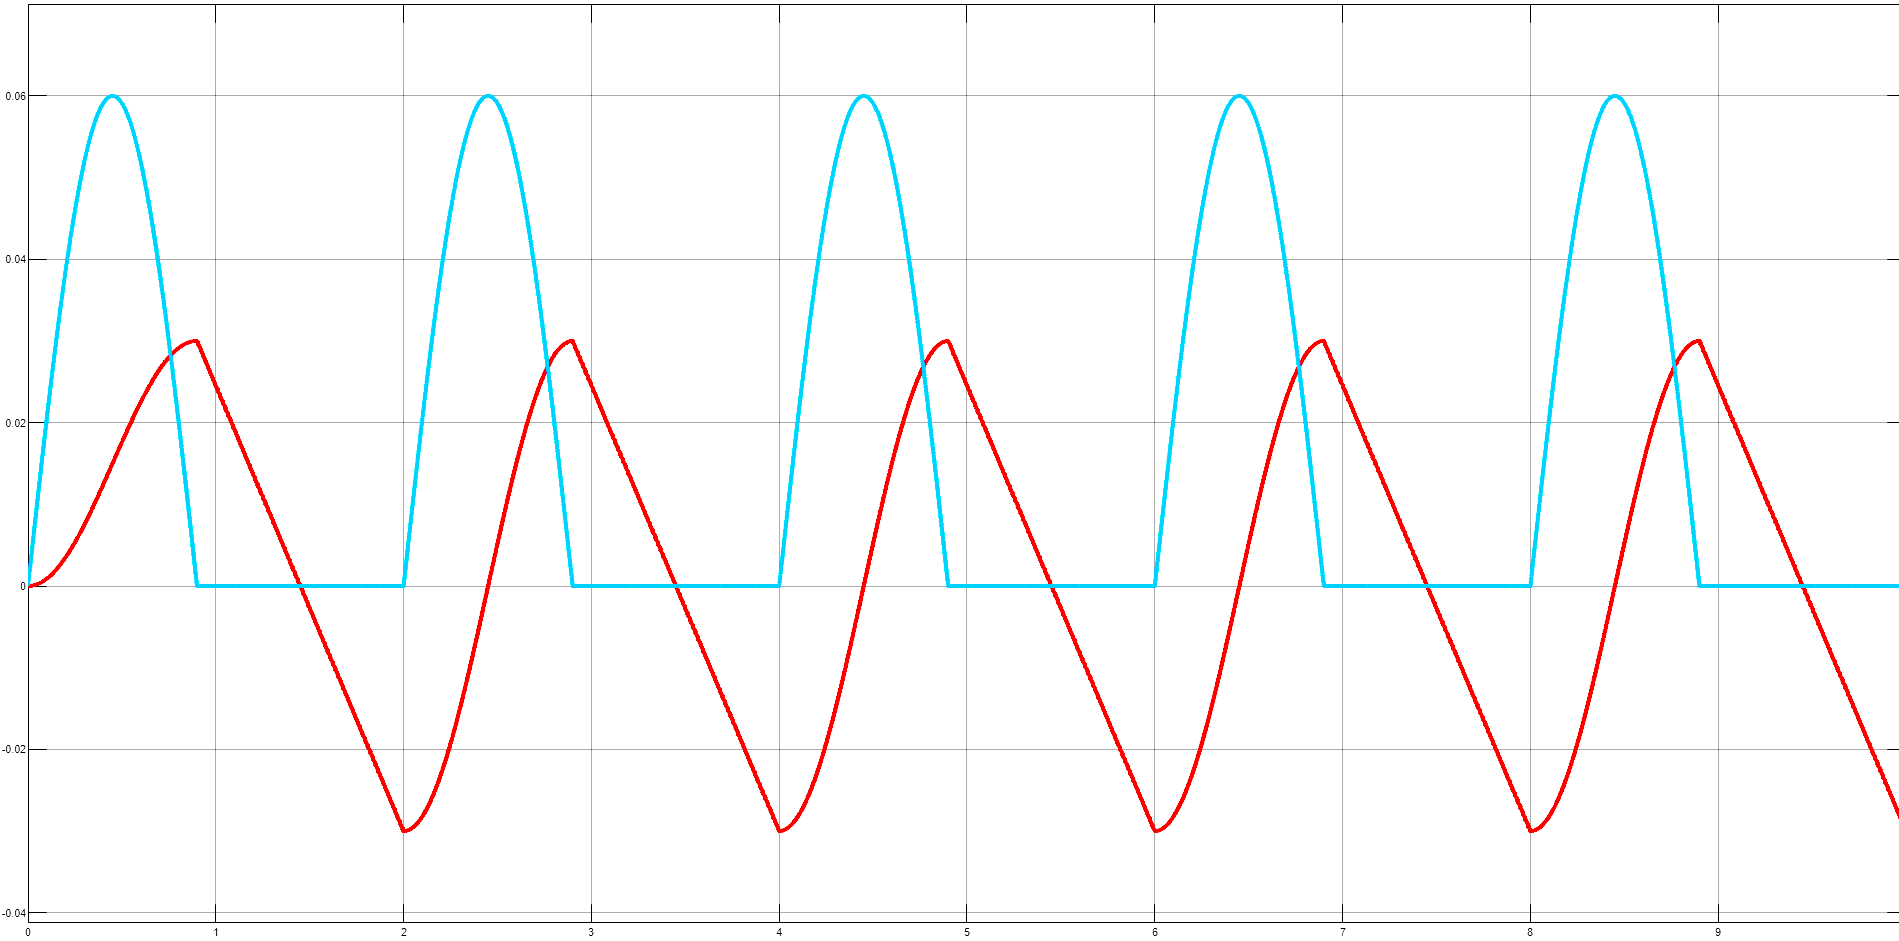
\includegraphics[scale=0.2]{Simulink/SignalGenerator_Graph_0.5Hz.PNG}}
	\caption{Trajectory coordinates generated by a signal generator with $f_c=0.5$\ Hz, $P_{Swing}=40\text{\%}$}
	\label{figure: Trajectory graphs}
\end{figure}

\begin{figure}[!h]
	\centering
	\begin{subfigure}[b]{0.55\textwidth}
		\includesvg[width=1\linewidth]{Simulink/Simulink_SwingPhaseGenOverview}
		\caption{}
		\label{fig:Ng1} 
	\end{subfigure}
	
	\begin{subfigure}[b]{0.55\textwidth}
	%	\includesvg[width=1\linewidth]{Simulink/Simulink_SwingPhaseGenOverview}
	\includegraphics[scale=0.5]{example-image-b}
		\caption{}
		\label{fig:Ng2}
	\end{subfigure}
	
	\caption[Swing and Stance Phase]{(a) Swing phase subsystem. The swing ellipse is generated by two sine waves with different amplitude and phase. (b) Stance phase subsystem. As opposed to (a), the x-coordinate is now generated by a linear function and the z-coordinate is 0 throughout the whole phase.}
\end{figure}


\subsubsection{Analytical Inverse Kinematics Solver} \label{subsubsec: IK Solver}
Even though Simulink's \textit{Robotics System Toolbox} includes an iterative inverse kinematics block, the block is not able to support the calculation speed we require.
The simulations, and thus the trajectory calculations as well, need to be run at about 1-2 kHz (time steps per second) to ensure stability of the simulation and smooth motion of the hexapod.
As we are not able to achieve this compute frequency with the provided numerical solver, we implement our own, purpose-build analytical IK solver aiming to drastically improve computation time.

\begin{figure}[!h]
	\begin{subfigure}{.5\textwidth} % this sets the figure to be max half the width of the page
		\centering
		% include first image
		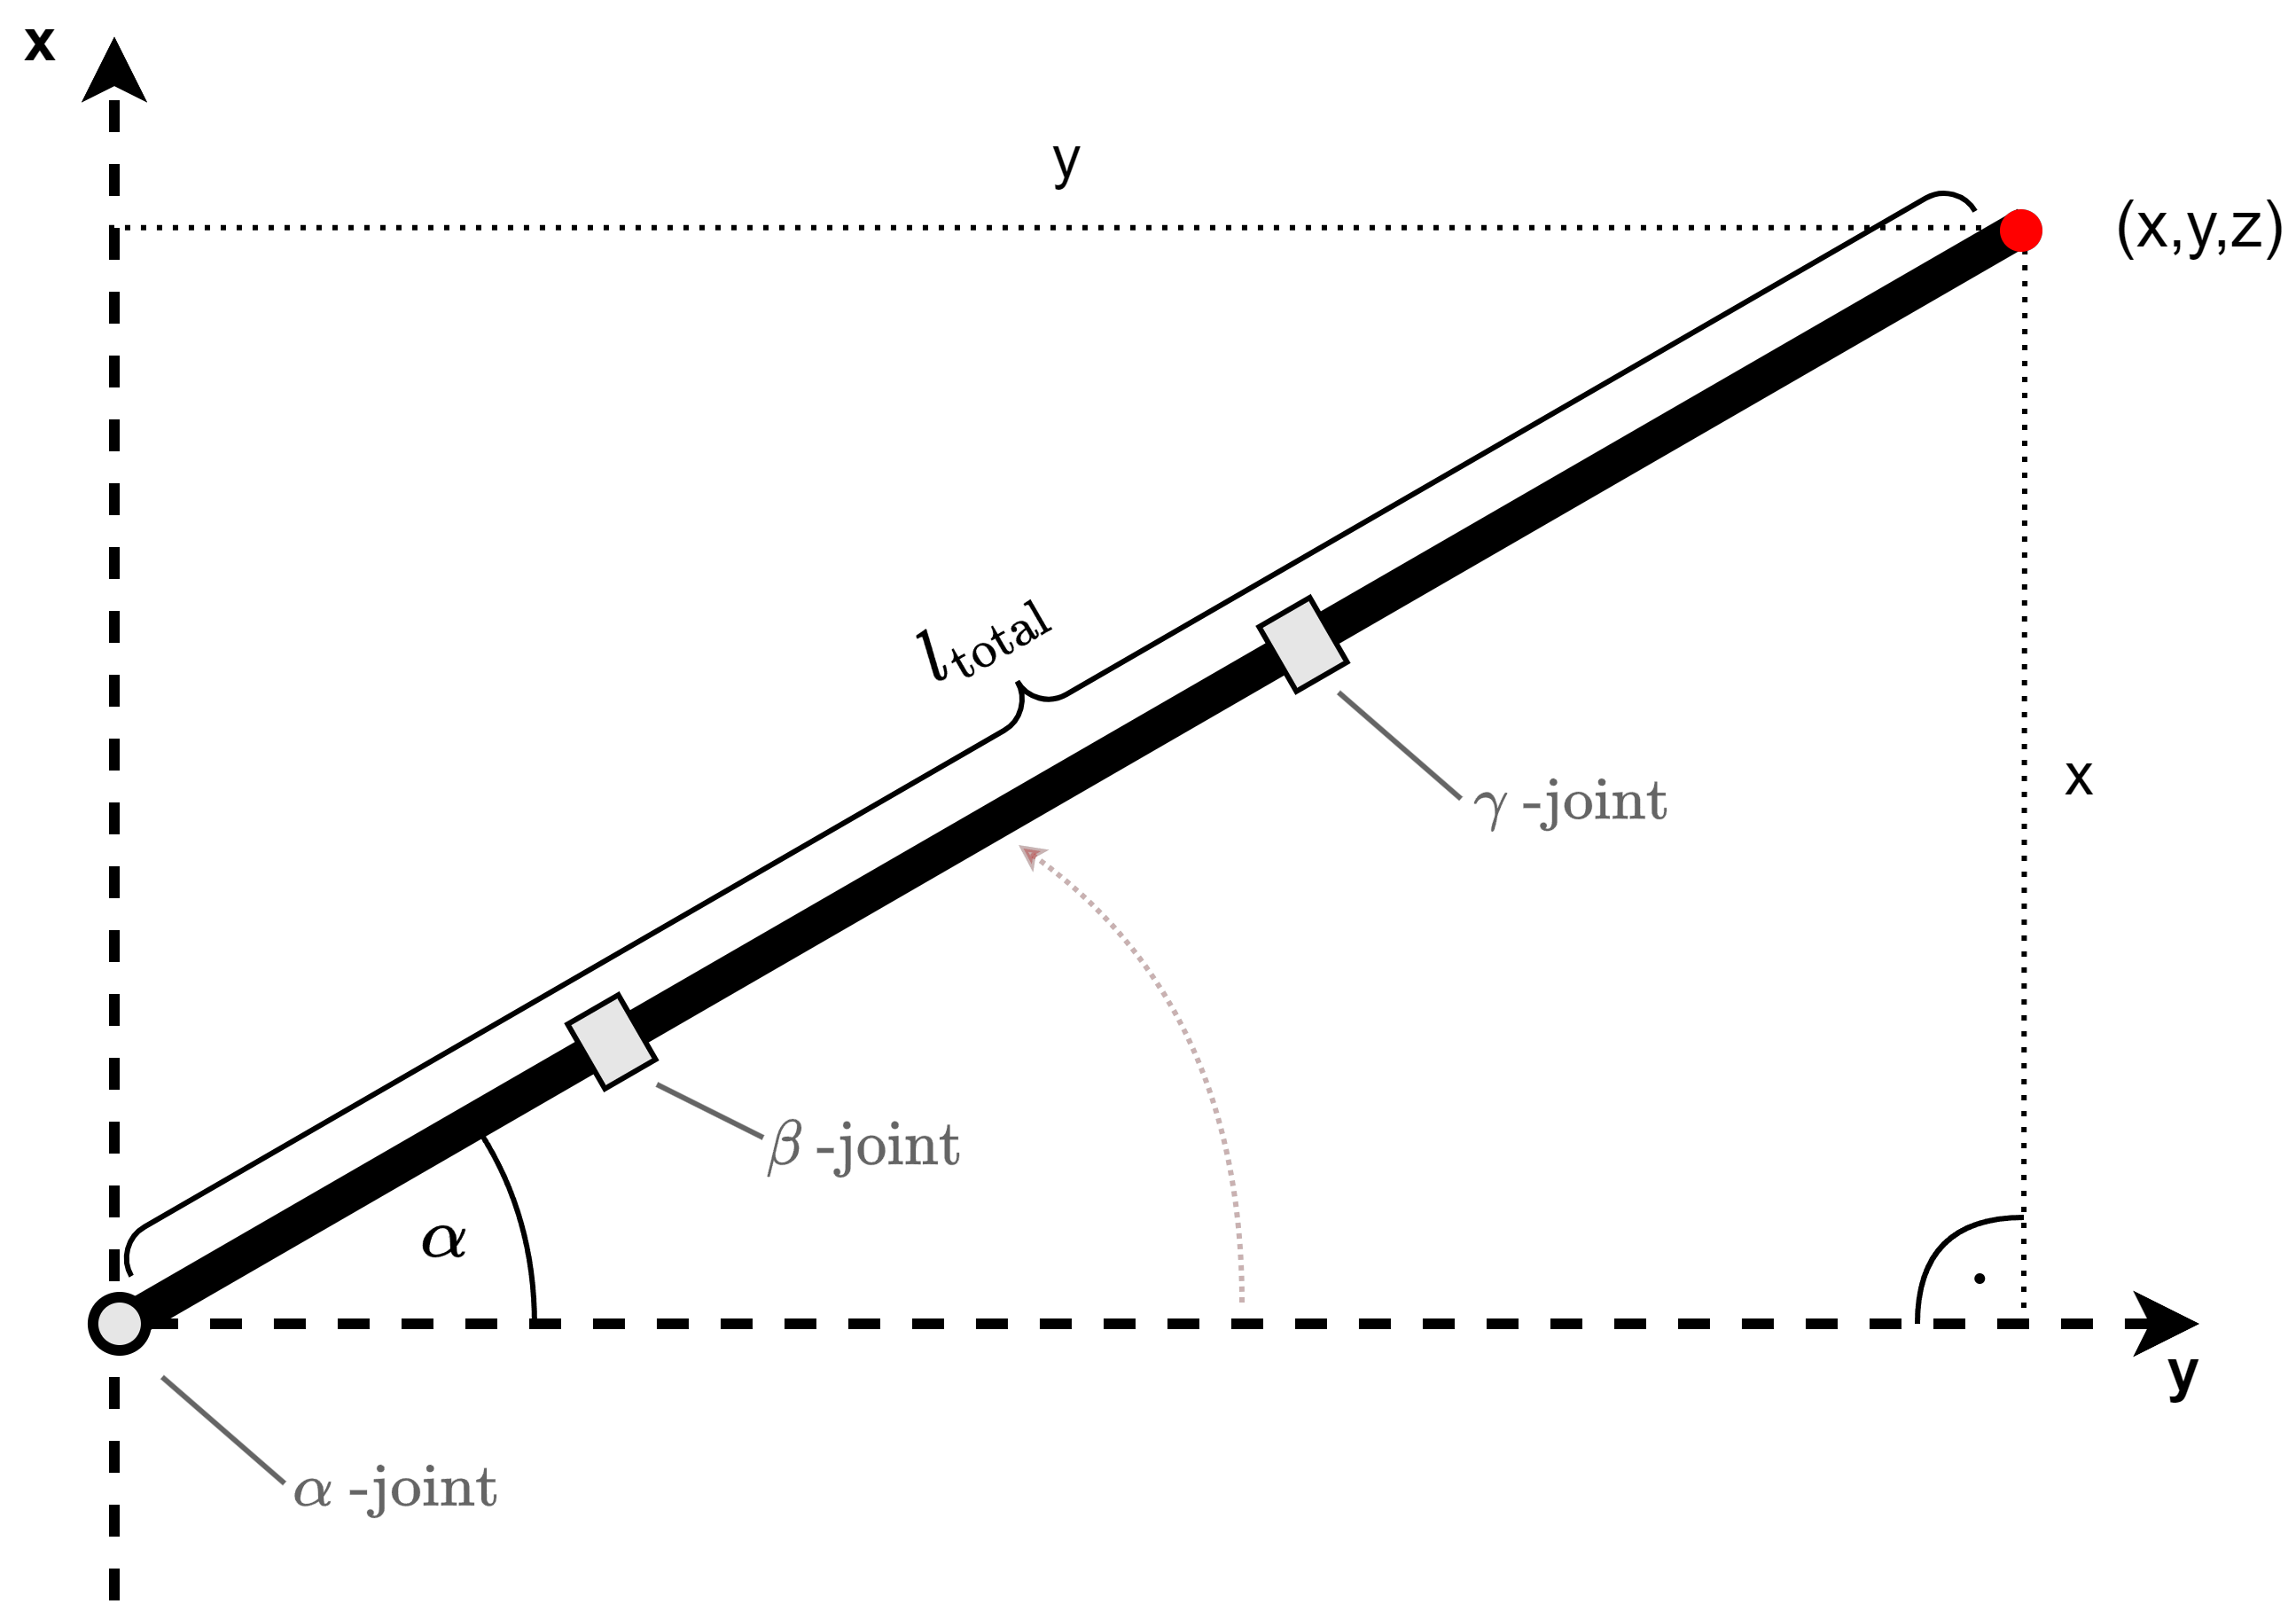
\includegraphics[width=.9\linewidth]{IK_Solver_alphaAngle}  % this sets the image to fill 90% of the available space -> 45% of the line width in total. 
		\caption{}
		\label{figure: IK Solver Alpha Angle}
	\end{subfigure}
	\begin{subfigure}{.5\textwidth}
		\centering
		% include second image
		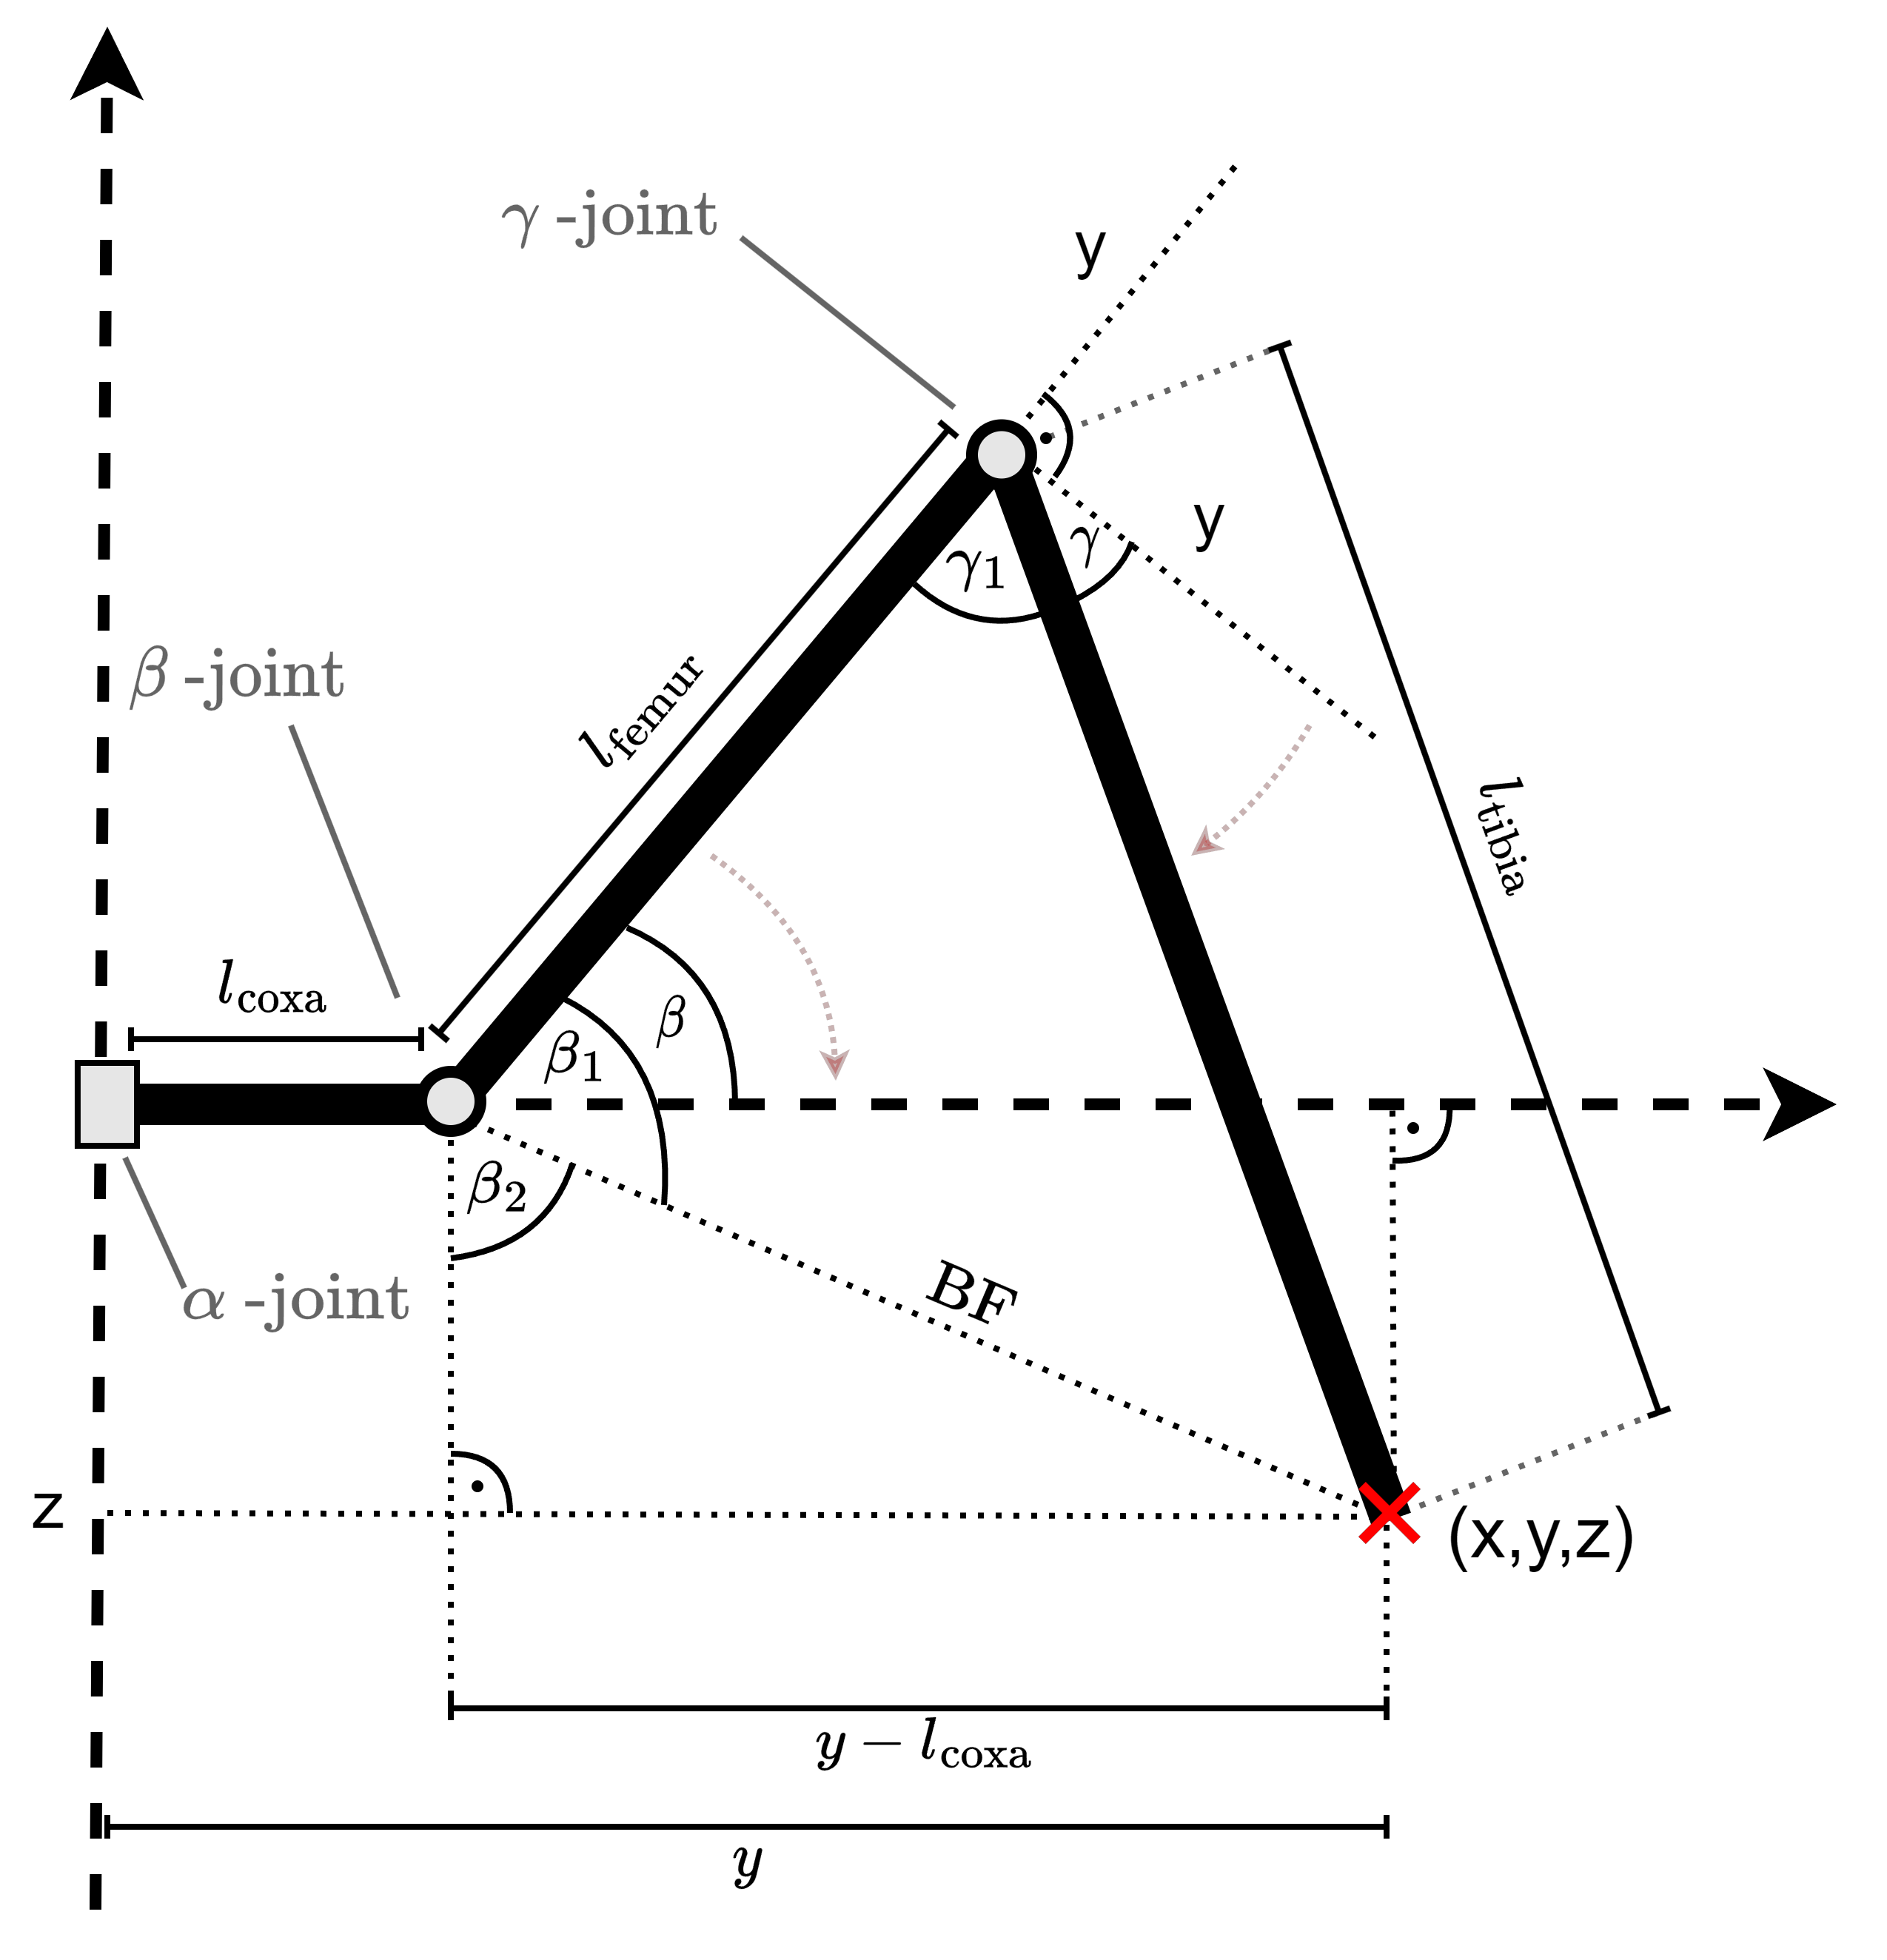
\includegraphics[width=.9\linewidth]{IK_Solver_betaGammaAngle}  
		\caption{}
		\label{figure: IK Solver Beta/Gamma Angle}
	\end{subfigure}
	\caption[Angle derivation drawings]{(a) Top-down view of a hexapod leg, used to determine \textalpha. (b) Side-view, used to calculate \textbeta \ and \textgamma.}
	\label{figure: IK angle derivations}
\end{figure}
\todo{Remove red cross in graphic, looks strange}

Our proposed solver sequentially calculates the legs joint angles, starting at \textalpha, then \textbeta \ and \textgamma.
We derive the following equations from the geometric properties of a hexapod leg as seen in \ref{figure: IK angle derivations}, translate them into C-code and run the resulting script inside a MATLAB code block.

\[
	\alpha = \arctan(\frac{x}{y}) ,\quad \quad \quad \beta = 90^{\circ} - (\beta_1 + \beta_2) ,\quad \quad \quad \gamma = 90^{\circ} - \gamma_1.
\]
\\
Where $\beta_1$, $\beta_2$, $\gamma_1$ and \text{BF} are given by:
\[	
	\beta_1 = \arccos(\frac{{l_\text{femur}}^2 + \text{BF}^2 - {l_\text{tibia}}^2}  {2\cdot l_\text{femur} \cdot \text{BF}}) ,\quad \quad \quad \beta_2 = \arctan(\frac{ l_\text{total} - l_\text{coxa}} {z}),
\]

\[
	\gamma_1 = \arccos(\frac{{l_\text{tibia}}^2 + {l_\text{femur}}^2 - {\text{BF}}^2}  {2 \cdot {l_\text{tibia}} \cdot {l_\text{femur}}}) ,\quad \quad \quad \text{BF} = \sqrt{(l_\text{total} - l_\text{coxa})^2 + z^2}.
\]

\begin{table}[h!]
	\centering
	\begin{tabular}{| c | c |}
		\hline
		parameter & value\\
		\hline
		\hline
		$K_p$ & 600 \\
		
		$K_i$ & 0.1 \\
		
		$K_d$ & 1 \\
		
		$N$ & 1000 \\
		\hline
	\end{tabular}
	\caption{Gain parameters used for PID-tuning}
	\label{table: PID parameters}
\end{table}

\begin{table}[h!]
	\centering
	\begin{tabular}{| c | c | c | c |} 
		\hline
		 & \textbf{\textalpha} & \textbf{\textbeta} & \textbf{\textgamma} \\ [0.5ex] 
		\hline
		\hline
		left front, right back & 45 & 14.03624347 & 60.58440117  \\ 
		
		left/right middle & 0 & 14.03624347 & 60.58440117 \\
		
		right front, left back & -45 & 14.03624347 & 60.58440117 \\
		\hline
	\end{tabular}
	\caption{Initial joint positions according to urdf-file}
	\label{table:Initial joint positions}
\end{table}
\todo{Muss keine Tabelle sein}


\section{Learning Leg Coordination} \label{sec: RL setup}
\todo{Redo this section}
From a RL point of view, the leg coordination problem can be considered a POMDP (Partially observable Markov decision process).
The POMDP is an extension to the MDP definition and describes problem spaces in which only parts of the environment can be observed.
This is particularly the case for complex continuous environments in which it is impossible to observe every detail of the process.
For the problem we try to solve here this holds true as well.

%The MDP is a 5-tuple $\mathcal{\{S,A,P,R,\gamma\}}$, where $\mathcal{S}$ is a finite set of states, $\mathcal{A}$ is a finite set of actions, $\mathcal{P}$ is a state-transition probability matrix ($\mathcal{P}_{ss'}^a=\mathbb{P}[S_{t+1}=s' | S_t=s, A_t=a]$), $\mathcal{R}_s^a$ is a reward function ($\mathcal{R}_s^a = \mathbb{E}[R_{t+1} | S_t=s, A_t=a]$) and $\gamma \in [0,1]$ is a discount factor.
We define the POMDP tuple $\mathcal{\{S,A,P,R,\gamma\}}$ as follows:
The state space $\mathcal{S}$ consists of all possible configurations of the continuous simulation environment and cannot be considered a finite set.\\
The action space $\mathcal{A}$ is defined as the set of all possible permutations of the action tuple $\{s_1,...,s_6\}$, meaning it is the set of all 6-bit binary numbers and thus is of size $2^6$.
It follows that the action space is discrete, as the agent can only decide to activate a swing phase or not.\\
As it is not required for the training process, we do not explicitly provide a state transition probability matrix $\mathcal{P}$.
The reward function $\mathcal{R}$ given by:
 \[
 R(t) = s_x(t) + v_x(t) - v_y(t) - \Delta_\text{h}(t) - 0.025 \cdot W(t) \ (+ r_\text{survival}).
 \]
\todo{Only current Def.}
The components of the reward functions are:
The distance $s_x(t)$ and speed $v_x(t)$ the robot walks along the x-axis, the speed $v_y(t)$ along the y-axis with which the robot deviates from its straight path, the height difference between the robots front and rear $\Delta_\text{h}(t)$, the energy consumption $W(t)$ and the survival reward $r_\text{survival}$.
By negatively rewarding height differences along the hexapods body as well as energy consumption, we aim to prevent undesirable jumping or twitching behaviour.
We experiment with several different discount factor $\gamma$, see chapter \ref{ch:results} for more information.

MATLABs Reinforcement Learning Toolbox offers several different RL architectures to choose from, namely DDPG, TR3, PPO, SAC and TRPO.
We choose to use the DDPG (Deep Deterministic Policy Gradient) as well as PPO (Proximal Policy Optimization) algorithms, as these have already proven themselves to work well in tasks concerning robotic locomotion\parencite{FIND AUTHOR}.
\todo{Find authors who used DDPG and PPO for robotics(PPO bei Schilling et al.(?), DDPG bei ? )}
To use such an agent in combination with a Simulink model, the model needs to include a \textit{RL agent} block from the \textit{Reinforcement Learning} toolbox.
One also has to define an observation and action space as well as an environment object in the MATLAB Workspace.
%There are 2 options for agent creation: The \textit{Reinforcement Learning Designer} MATLAB app with a reduced graphical interface or a MATLAB script-file in which the agent is defined in detail.
We choose the utilise MATLAB scripts for this purpose, as this allows us to permanently specify agents and also automate the agent creation task.
For each of the agents we experimented with, DDPG, continuous and discrete PPO, we write a separate creation script.
\todo{Expand}

To speed up the learning process, we decided to utilize \textit{MATLABs Parallel Computing} toolbox.
The toolbox allows us to initialise a parallel pool of several workers, each of whom runs a separate episode of the RL training process.
The parallel learning process is carried out asynchronously, meaning workers who finish their task early do not have to wait on the others to finish as well before proceeding.
In contrast to synchronous parallelization, where the workers send their results to the parallel pool client all at the same time and receive updates to their parameters all at once, workers under asynchronous parallelization can send their results as soon as they finish their task and instantly receive parameter updates.
%By parallelization, we significantly improve the number of simulated episodes.



We start the training of agents at a small simulation step size(0.00025s = 0.25ms) to prevent simulation errors due to initial random jerking of robot legs.
After the agent has stabilized, the step size is increased to speed up the further learning process.
\cite{lillicrap2015continuous}




\textbf{Optionals:}

\begin{itemize}
	\item Signal the agent that a leg is dragging by adding a discrete observation per leg which is pulled high when the leg reached its PEP.
	
	\item Add more inputs to the RL agent $\rightarrow$ Done, added accelerations
	
	\item Agent Parallelization for faster learning $\rightarrow$ Done and working
	
	\item RL Designer: Automatically save agents which reach a high enough reward to evaluate them later $\rightarrow$ Done.
	
	\item As we have multiple robotic 'actuators' in this project, a continuous action space is favorable $\rightarrow$ Not the case, as we have discrete actions
	
\end{itemize}




